% !TEX root = ../../../main.tex
% 所属：第二部分：多变量分析学 / 第3章：重积分
% 节：3.1 有界闭区域上的重积分
% 正文按原文件顺序保存；由 ../chapter3.tex 调用。
\section{有界闭区域上的重积分}

\subsection*{Riemann 意义下的平面面积}

设 $D$ 为 $\R^2$ 上的有界子集，设
$U=[a,b]\times[c,d]$ 为包含 $D$ 的一个闭矩形。
在 $[a,b]$ 中插入分点
\[
a=x_0<x_1<\cdots<x_n=b,
\]
在 $[c,d]$ 中插入分点
\[
c=y_0<y_1<\cdots<y_m=d.
\]
这些分点作平行于坐标轴的直线，将 $U$ 分成许多小矩形
\[
U_{ij}=[x_{i-1},x_i]\times[y_{j-1},y_j],
\qquad i=1,2,\ldots,n,\quad j=1,2,\ldots,m.
\]
这称为 $U$ 的一个划分。把完全包含于 $D$ 内的那些小矩形的面积之和
记为 $mA$，与 $D$ 的交集非空的那些小矩形的面积之和记为 $mB$，
则显然它们与 $U$ 的划分有关，且有 $mA\le mB$。

\begin{center}
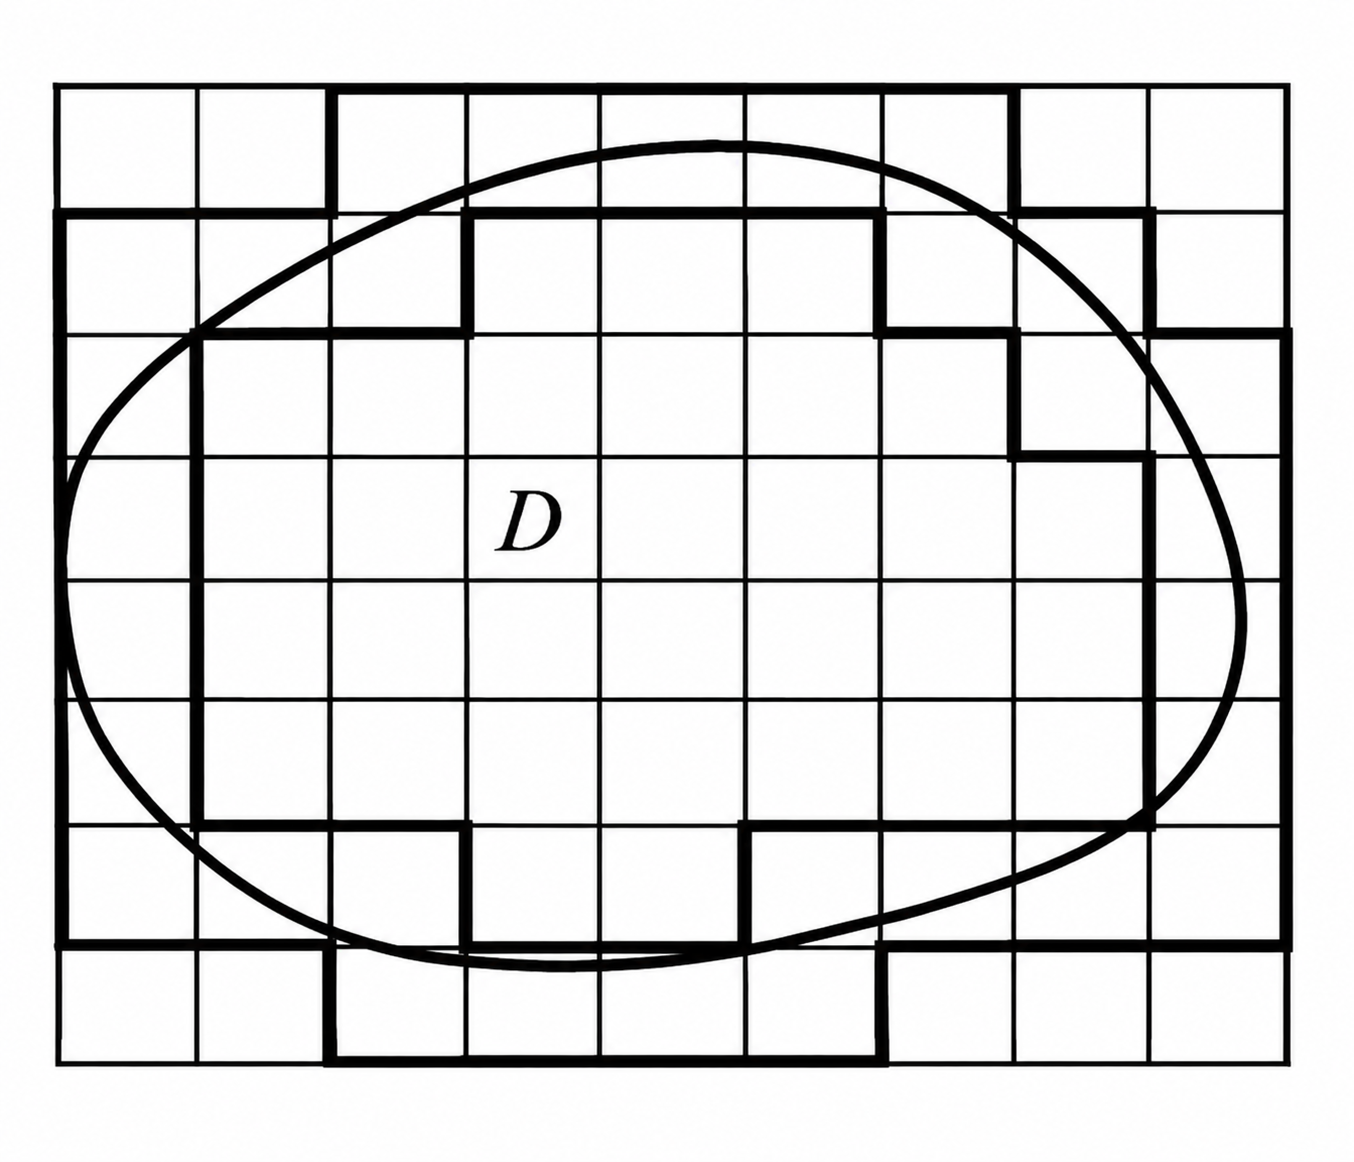
\includegraphics[width=0.29\textwidth]{figure/P2/fig13_1_1_source_hd.png}
\end{center}



\begin{proposition}\label{p2-area-refinement-comparison}
若在原有划分的基础上，在 $[a,b]$ 和 $[c,d]$ 中再增加有限个分点
（所得的新划分称为原来划分的加细），则 $mB$ 不增，$mA$ 不减；
且任意一种划分所得到的 $mA$ 不大于任意另一种划分所得到的 $mB$。
\end{proposition}
\begin{proof}
记划分 $P$ 所对应的两个面积和为 $mA(P)$ 与 $mB(P)$。
先只在一个坐标区间内增加一个分点，
得到加细后的划分 $P'$。此时每个被新分割线切到的原小矩形 $Q$
分为两个小矩形 $Q_1,Q_2$，且 $|Q|=|Q_1|+|Q_2|$。

若 $Q\subset D$，则 $Q_1,Q_2\subset D$，加细前后它对 $mA$
的贡献相等；若 $Q\not\subset D$，它原来对 $mA$ 的贡献为零，
加细后的贡献非负。因此 $mA(P)\le mA(P')$。
另一方面，若 $Q\cap D=\varnothing$，则 $Q_1,Q_2$ 均不与 $D$ 相交；
若 $Q\cap D\ne\varnothing$，加细后它们对 $mB$ 的贡献之和
至多为 $|Q_1|+|Q_2|=|Q|$。因此 $mB(P')\le mB(P)$。
依次增加有限个分点，就得到第一部分的结论。

现任取两个划分 $P_1,P_2$，将它们在两个坐标区间内的分点分别合并，
得到共同加细 $P^*$。由刚证明的单调性，以及同一划分下
$mA(P^*)\le mB(P^*)$，有
\[
mA(P_1)\le mA(P^*)\le mB(P^*)\le mB(P_2).
\]
所以任意一个 $mA$ 都不大于任意一个 $mB$。
\end{proof}


\begin{definition}
	$mA$ 有一个上确界 $mD_*$，
$mB$ 有一个下确界 $mD^*$，并且
\[
mD_*\le mD^*.
\]
若 $mD_*=mD^*$，则称这个值为 $D$ 的面积，记为 $mD$，
此时称 $D$ 是\textbf{可求面积的}。显然 $D$ 的面积与 $U$ 的选取无关。
\end{definition}

同样可以考虑 $D$ 的边界 $\partial D$ 的面积：
记与 $\partial D$ 的交集非空的那些小矩形的面积之和为
$mB_{\partial D}$。若 $mB_{\partial D}$ 的下确界
$mD^*_{\partial D}=0$，则称 $\partial D$ 的面积为零；
边界的面积为零等价于所围区域是可求面积的区域。
对任意给定的 $\varepsilon>0$，通过取足够细的划分，
可使得
\[
mB-mA=mB_{\partial D}<\varepsilon.
\]
那么就有以下的判据：
\begin{proposition}(Jordan 可求面积判据)
有界点集 $D$ 是可求面积的充分必要条件是它的边界
$\partial D$ 的面积为 $0$。
\end{proposition}

因此，零边界围成的区域是可求面积的。

面积具有可加性：如果有界点集 $D$ 由点集 $D_1$ 和 $D_2$ 组成，
$D_1$ 和 $D_2$ 可求面积，且 $D_1\cap D_2=\varnothing$，
那么 $D$ 可求面积，并满足
\[
mD=mD_1+mD_2.
\]

\begin{example}
设 $y=f(x)$（$a\le x\le b$）为非负连续函数，
它与直线 $x=a$、$x=b$ 和 $y=0$ 所围成的区域
\[
D=\{(x,y):a\le x\le b,\ 0\le y\le f(x)\}
\]
是可求面积的。

\begin{center}
% 图 13.1.2：曲线 y=f(x) 下的曲边梯形。
\begin{tikzpicture}[x=0.82cm,y=0.82cm,>=Stealth,baseline=(current bounding box.center)]
  \draw[->,line width=0.45pt] (-0.18,0) -- (5.65,0) node[right,font=\scriptsize] {$x$};
  \draw[->,line width=0.45pt] (0,-0.2) -- (0,3.35) node[above,font=\scriptsize] {$y$};
  \node[below left,font=\scriptsize] at (0,0) {$O$};
  \draw[line width=0.65pt] (0.9,0) -- (0.9,1.75);
  \draw[line width=0.65pt] (5.0,0) -- (5.0,3.05);
  \draw[line width=0.8pt]
    (0.9,1.75) .. controls (0.86,2.12) and (1.1,2.32) .. (1.55,2.44)
    .. controls (2.65,2.72) and (3.95,2.55) .. (4.52,2.73)
    .. controls (4.78,2.84) and (4.93,2.99) .. (5.0,3.05);
  \node[above,font=\scriptsize] at (3.05,2.69) {$y=f(x)$};
  \node[font=\scriptsize] at (2.85,1.2) {$D$};
  \node[below,font=\scriptsize] at (0.9,0) {$a$};
  \node[below,font=\scriptsize] at (5.0,0) {$b$};
\end{tikzpicture}

\end{center}

\begin{proof}
由于 $f$ 在 $[a,b]$ 上连续，那么在 $[a,b]$ 上可积。
记 $m=\min\limits_{x\in[a,b]}f(x)$，
$M=\max\limits_{x\in[a,b]}f(x)$。
若 $M=0$，则 $f\equiv0$，此时 $D=[a,b]\times\{0\}$
可用面积任意小的矩形覆盖，故面积为零，结论成立。
以下设 $M>0$。
在 $[a,b]$ 上插入分点
$a=x_0<x_1<\cdots<x_n=b$，
将 $[a,b]$ 等分，记 $h_n=(b-a)/n$；
那么矩形 $U=[a,b]\times[0,M]$ 就包含了区域 $D$。
按一元积分的 Darboux 和，令 $m_i,M_i$ 分别为
$f(x)$ 在 $[x_{i-1},x_i]$ 上的最小值与最大值。
在 $[0,M]$ 上插入分点
$m_i,M_i$（$i=1,\ldots,n$），合并重复分点后，
就得到 $U$ 的一个划分 $P_n$。
容易看出，包含于 $D$ 内的那些小矩形的面积之和为
\[
mA(P_n)=\sum_{i=1}^n m_i h_n.
\]

记 $\omega_n=\max\limits_{1\le i\le n}(M_i-m_i)$。
由 $f$ 在 $[a,b]$ 上的一致连续性，$\omega_n\to0$。
又因 $f([a,b])=[m,M]$，在 $[m,M]$ 中任意两个相邻的
$y$ 向分点 $s<t$ 都满足 $t-s\le\omega_n$。
事实上，任取 $z\in(s,t)$，存在 $x\in[a,b]$ 使 $f(x)=z$。
若 $x\in[x_{k-1},x_k]$，则 $m_k\le z\le M_k$；
由于 $m_k,M_k$ 都是分点，且 $(s,t)$ 内没有分点，
故 $m_k\le s<t\le M_k$，从而 $t-s\le M_k-m_k\le\omega_n$。

在第 $i$ 个竖条中，上边缘的纵坐标不超过 $M_i$ 的小矩形均与 $D$ 相交。
若 $M_i<M$，紧邻 $M_i$ 上方的小矩形也因在边界上与 $D$ 相交而被计入
$mB(P_n)$，但其高度至多为 $\omega_n$；
其余位于 $M_i$ 上方的小矩形不与 $D$ 相交。
因此应有估计
\[
\sum_{i=1}^n M_i h_n
\le mB(P_n)
\le\sum_{i=1}^n M_i h_n+(b-a)\omega_n.
\]
于是
\[
\sum_{i=1}^n m_i h_n
\le mD_*\le mD^*
\le\sum_{i=1}^n M_i h_n+(b-a)\omega_n.
\]
令 $n\to\infty$，由 $f$ 在 $[a,b]$ 上的可积性及极限的夹逼性得
\[
mD_*=mD^*=\int_a^b f(x)\,\dd x.
\]
因此 $D$ 是可求面积的，且面积为
$\displaystyle\int_a^b f(x)\,\dd x$。

这里证明面积存在，只需使 $mB(P_n)-mA(P_n)\to0$，
不要求划分 $P_n$ 的模长趋于零。
当 $m>0$ 时，底部区间 $[0,m]$ 无须再等分，
因为对应的小矩形完全包含于 $D$，对 $mA(P_n)$ 与 $mB(P_n)$ 的贡献相同。
\end{proof}

\textbf{注记：}按前面的定义，小矩形只要与 $D$ 的交集非空，其整个面积就计入 $mB$。
因此，仅在边界上与 $D$ 相交的闭矩形也会被计入，一般不能直接写成
$mB=\sum\limits_i M_i\Delta x_i$。
例如，取 $f(x)=x$（$0\le x\le1$），两条坐标轴上都取分点 $0,\frac12,1$，
则左上角的小矩形仅在点 $(\dfrac12,\dfrac12)$ 处与 $D$ 相交，但其面积仍被计入。
此时 $mB=1$，而 Darboux 上和为 $\dfrac34$。
\end{example}

在上述例中，记曲线 $y=f(x)$（$a\le x\le b$）为 $L$。
覆盖 $L$ 的那些小矩形
$[x_{i-1},x_i]\times[m_i,M_i]$ 的面积之和为
\[
\sum_{i=1}^n(M_i-m_i)(x_i-x_{i-1}).
\]
当 $n\to\infty$ 时，它的极限是零(由一致连续性证得)，所以曲线的面积为零。
可以用同样方法进一步证明：

平面上一条光滑曲线的面积为零。
因此，若一个有界区域的边界是分段光滑曲线，
那么它是可求面积的。

注意，并不是所有开平面点集都是可求面积的。
例如平面点集
\[
S=\{(x,y):0\le x\le1,\ 0\le y\le D(x)\},
\qquad
D(x)=
\begin{cases}
1,&x\text{ 为有理数},\\
0,&x\text{ 为无理数},
\end{cases}
\]
其中 $D(x)$ 是 Dirichlet 函数。
$S$ 的边界为 $[0,1]\times[0,1]$，它的面积为 $1$，
这说明 $S$ 不是可求面积的。

\subsection*{二重积分的概念}

考察一个曲顶柱体：它的底是 $xy$ 平面上的具有零边界的
有界闭区域 $D$，顶是非负连续函数 $z=f(x,y)$，
$(x,y)\in D$ 所确定的曲面，侧面是以 $D$ 的边界曲线为准线、
母线平行于 $z$ 轴的柱面。

\begin{center}
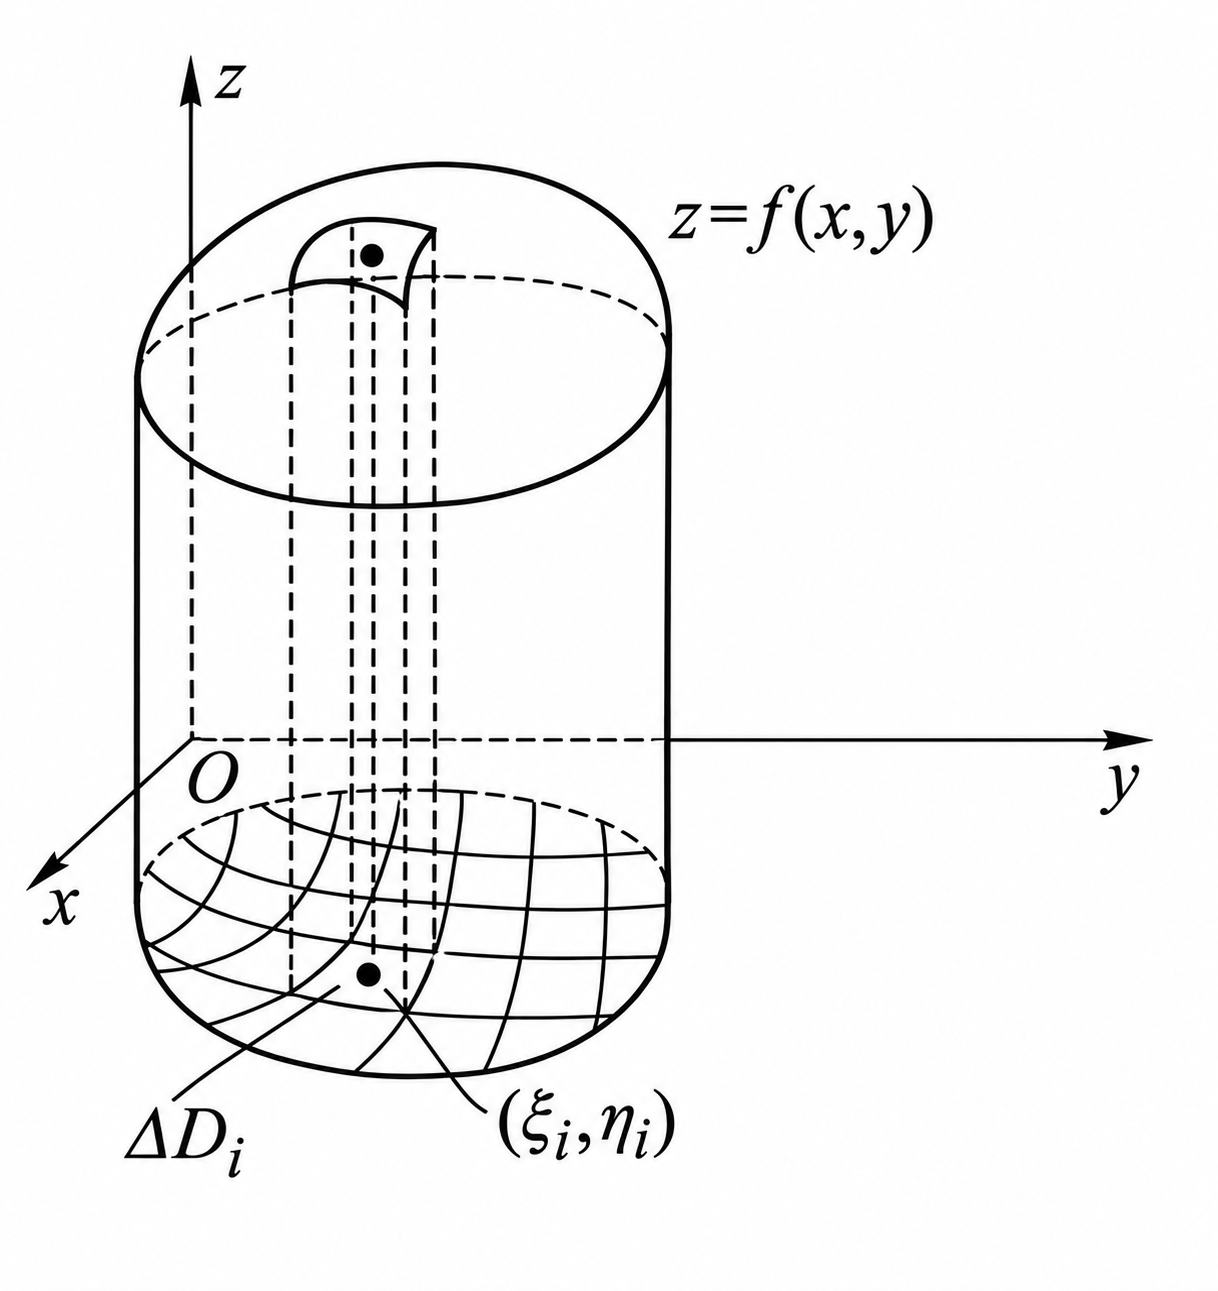
\includegraphics[width=0.34\textwidth]{figure/P2/fig13_1_3_source_hd.png}
\end{center}

为了求出它的体积 $V$，先用一些面积为零的曲线段组成的曲线网
将区域 $D$ 分成 $n$ 个小区域
$\Delta D_1,\Delta D_2,\ldots,\Delta D_n$。
由前面的讨论，每个 $\Delta D_i$ 都是可求面积的
（$i=1,2,\ldots,n$）。
再分别以这些小区域的边界为准线，作母线平行于
$z$ 轴的柱面，这些柱面将原曲顶柱体分成 $n$ 个细的小曲顶柱体。
在每个 $\Delta D_i$ 上任取一点 $(\xi_i,\eta_i)$，
那么以 $\Delta D_i$ 为底的小曲顶柱体的体积近似地等于
\[
f(\xi_i,\eta_i)\Delta\sigma_i,
\]
这里 $\Delta\sigma_i$ 表示 $\Delta D_i$ 的面积。
于是，原曲顶柱体的体积近似地等于
\[
\sum_{i=1}^n f(\xi_i,\eta_i)\Delta\sigma_i.
\]
当所有小区域 $\Delta D_i$ 的最大直径（记为 $\lambda = \max \limits_{1\leqslant k \leqslant  n}\operatorname{diam}\Delta_k$）
趋于零时，这个近似值趋于原曲顶柱体的体积，即
\[
V=\lim_{\lambda\to0}
\sum_{i=1}^n f(\xi_i,\eta_i)\Delta\sigma_i.
\]
这就是二重积分的概念。
以下讨论积分存在性时，总假定区域的边界以及
用来分割区域的曲线段的面积为零，
这就保证了所涉及的一切区域的面积都存在。

\begin{definition}[二重积分]
设 $D$ 为 $\R^2$ 上的\textbf{零边界闭区域}，函数 $z=f(x,y)$ 在 $D$ 上有界。
将 $D$ 用曲线网分成 $n$ 个小区域
$\Delta D_1,\Delta D_2,\ldots,\Delta D_n$
（它称为 $D$ 的一个划分），并记所有小区域
$\Delta D_i$ 的最大直径为
\[
\lambda=\max_{1\le i\le n}|\operatorname{diam}\Delta D_i|.
\]
在每个 $\Delta D_i$ 上任取一点 $(\xi_i,\eta_i)$，
记 $\Delta\sigma_i$ 为 $\Delta D_i$ 的面积。
若 $\lambda$ 趋于零时，和式
\[
\sum_{i=1}^n f(\xi_i,\eta_i)\Delta\sigma_i
\]
的极限存在，且与区域的分法和点
$(\xi_i,\eta_i)$ 的取法无关，
则称 $f(x,y)$ 在 $D$ 上可积，并称此极限为
$f(x,y)$ 在 $D$ 上的\textbf{二重积分}，记为
\[
\iint_D f(x,y)\,\dd\sigma
=\lim_{\lambda\to0}
\sum_{i=1}^n f(\xi_i,\eta_i)\Delta\sigma_i.
\]
$f(x,y)$ 称为被积函数，$D$ 称为积分区域，
$x$ 和 $y$ 称为积分变量，$\dd\sigma$ 称为面积元素，
$\displaystyle\iint_D f(x,y)\,\dd\sigma$ 也称为积分值。
\end{definition}

用 $\varepsilon$-$\delta$ 语言，上述定义是：
对任意 $\varepsilon>0$，存在 $\delta>0$，
使对任意划分 $P$ 及任意选点 $ \vect q_i\in\Delta D_i$，
只要 $\lambda(P)<\delta$，就有
\[
\left|\sum_i f(\vect q_i)\Delta\sigma_i-I\right|<\varepsilon.
\]
这里 $I$ 为同一个常数，$\delta$ 不依赖于划分及选点。

前面提到的曲顶柱体的体积即为
\[
V=\iint_D f(x,y)\,\dd\sigma.
\]

与一元的情况类似，下面用 Darboux 和讨论二重积分的可积性。
以下始终设 $D$ 为有界零边界闭区域，$f$ 在 $D$ 上有界，
记 $\sigma=mD$。
划分 $P=\{\Delta D_1,\ldots,\Delta D_n\}$ 中各小区域取为闭的小块，
其内部互不相交，公共边界的面积为零，因而
\[
\sum_{i=1}^n\Delta\sigma_i=\sigma,
\qquad
\lambda(P)=\max_{1\le i\le n}\operatorname{diam}\Delta D_i.
\]
非空的零面积小块也可保留在划分中，它们对各和式的贡献为零。
两划分合并曲线网所得的共同加细，可用原有小块的非空交集表示；
若交集分成多个小区域，对它们的贡献求和即可。
这些子块的边界仍包含于原有零面积边界的并集中。
用矩形网与 $D$ 相交，可得到模长任意小的划分。

设
\[
M_i=\sup_{\Delta D_i}f,\qquad
m_i=\inf_{\Delta D_i}f,\qquad
\omega_i=M_i-m_i,
\]
定义 Darboux 大和、小和分别为
\[
S(P)=\sum_{i=1}^n M_i\Delta\sigma_i,\qquad
s(P)=\sum_{i=1}^n m_i\Delta\sigma_i.
\]
其中 $\omega_i$ 称为 $f$ 在 $\Delta D_i$ 上的振幅。
在各小块中任取点 $\vect q_i=(\xi_i,\eta_i)$，
相应的 Riemann 和记为
\[
J(P;\vect q)=\sum_{i=1}^n f(\vect q_i)\Delta\sigma_i,
\qquad
s(P)\le J(P;\vect q)\le S(P).
\]

沿用命题 \ref{p2-area-refinement-comparison} 中逐块估计和共同加细的论证，
可得 Darboux 和的相应性质：
加细后，各子块的上确界不大于原小块的上确界，
下确界不小于原小块的下确界；再由面积的可加性，
若 $P'$ 是 $P$ 的加细，就有
\[
s(P)\le s(P')\le S(P')\le S(P).
\]
任取两个划分 $P_1,P_2$，将它们合并为共同加细 $P^*$，则
\[
s(P_1)\le s(P^*)\le S(P^*)\le S(P_2).
\]
所以任何一个 Darboux 小和都不大于任何一个 Darboux 大和。
记 $m=\inf_D f$、$M=\sup_D f$，还有
\[
m\sigma\le s(P_1)\le S(P_2)\le M\sigma.
\]
因此，由实数的确界存在定理，所有 Darboux 小和的上确界
与所有 Darboux 大和的下确界都存在。
分别称
\[
I_*=\sup_P s(P),\qquad I^*=\inf_P S(P)
\]
为 $f$ 在 $D$ 上的\textbf{下积分}和\textbf{上积分}。
这里的确界取遍本节定义所允许的全部划分 $P$，
不涉及小块内选点的取法，也不要求预先知道 $f$ 可积。
上、下积分可能不相等，但对任意划分 $P$ 都有
\[
m\sigma\le s(P)\le I_*\le I^*\le S(P)\le M\sigma.
\]

% 对应第一部分命题 8.3.8。
\begin{proposition}[二重积分的 Darboux 定理]\label{p2-darboux-limit}
当划分的模长 $\lambda(P)\to0$ 时，
\[
S(P)\to I^*,\qquad s(P)\to I_*.
\]
即对任意 $\varepsilon>0$，存在 $\delta>0$，
使得对任意划分 $P$，只要 $\lambda(P)<\delta$，就有
\[
0\le S(P)-I^*<\varepsilon,\qquad
0\le I_*-s(P)<\varepsilon.
\]
\end{proposition}
\begin{proof}
先说明任意充分细的划分与一个固定划分合并时，和式的变化可以任意小。
固定 $P_0=\{E_1,\ldots,E_r\}$，记
\[
\Gamma=\bigcup_{j=1}^r\partial E_j.
\]
由于区域边界和分割曲线的面积为零，$\Gamma$ 是面积为零的紧集。
任给 $\alpha>0$，可用有限个开矩形覆盖 $\Gamma$，
使其面积之和小于 $\alpha$；记这些开矩形的并为 $G$。
由 $\Gamma$ 的紧性，存在 $\rho>0$，使
\[
\Gamma_\rho=\{z:\operatorname{d}(z,\Gamma)<\rho\}\subset G.
\]

设 $P^*$ 为 $P,P_0$ 的共同加细。
把 $P$ 中不包含于任何一个 $E_j$ 的小块称为受影响的小块。
若 $\lambda(P)<\rho/2$，则每个受影响的小块都包含于 $G$。
事实上，任取其中一点 $p$，选取含 $p$ 的 $E_j$；
由于该小块不包含于 $E_j$，其中还存在 $q\notin E_j$。
线段 $pq$ 必经过 $\partial E_j$ 上某点 $z$，
于是对该小块中任意点 $w$，
\[
|w-z|\le |w-p|+|p-z|
\le 2\lambda(P)<\rho.
\]
所以该小块包含于 $\Gamma_\rho$。
各小块只在零面积边界上重叠，故受影响小块的面积之和 $A(P)$ 满足
\[
A(P)\le mG<\alpha.
\]

记 $K=M-m$。未受影响的小块在共同加细前后贡献不变，
受影响小块的上、下和变化分别不超过 $K$ 乘以该小块的面积，故
\[
\begin{aligned}
0&\le S(P)-S(P^*)\le K A(P),\\
0&\le s(P^*)-s(P)\le K A(P).
\end{aligned}
\]
因此对固定的 $P_0$，上述两种变化都随 $\lambda(P)\to0$ 而趋于零。

现证明 $S(P)\to I^*$。
任给 $\varepsilon>0$，由下确界的定义，可取固定划分 $P_0$，使
\[
0\le S(P_0)-I^*<\frac{\varepsilon}{2}.
\]
在前面的估计中取 $\alpha=\varepsilon/[2(K+1)]$，
并取相应的 $\delta=\rho/2$。
当 $\lambda(P)<\delta$ 时，
\[
\begin{aligned}
0\le S(P)-I^*
&=S(P)-S(P^*)+S(P^*)-I^*\\
&\le K A(P)+S(P_0)-I^*
<\varepsilon.
\end{aligned}
\]
同理，由上确界的定义，先取 $s(P_0)>I_*-\varepsilon/2$，
再用 $s(P^*)\ge s(P_0)$，即可得到 $0\le I_*-s(P)<\varepsilon$。
\end{proof}

% 对应第一部分命题 8.3.9。
\begin{proposition}[上下积分相等判据]\label{p2-integrability-upper-lower}
$f$ 在 $D$ 上可积的充分必要条件是 $I_*=I^*$。
此时
\[
\iint_D f(x,y)\,\dd\sigma=I_*=I^*.
\]
\end{proposition}
\begin{proof}
必要性：设 $f$ 可积，积分值为 $I$。
任给 $\varepsilon>0$，由积分定义，存在 $\delta>0$，
使得当 $\lambda(P)<\delta$ 时，对任意选点 $\vect q_i$ 都有
\[
|J(P;\vect q)-I|<\varepsilon.
\]
对这样的划分，由上确界的定义，可以逐块选取 $\vect q_i^+$，使
\[
M_i-\frac{\varepsilon}{\sigma+1}<f(\vect q_i^+)\le M_i.
\]
于是
\[
0\le S(P)-J(P;\vect q^+)\le
\frac{\varepsilon\sigma}{\sigma+1}<\varepsilon,
\]
故 $|S(P)-I|<2\varepsilon$。
同理，逐块选取逼近下确界的点，得到 $|s(P)-I|<2\varepsilon$。
结合命题 \ref{p2-darboux-limit}，可知 $I^*=I_*=I$。
这里不要求上、下确界能在小块中取到。

充分性：设 $I_*=I^*=I$。
由命题 \ref{p2-darboux-limit}，当 $\lambda(P)\to0$ 时，
$s(P),S(P)$ 都趋于 $I$。
而任意选点所得的 Riemann 和都满足
\[
s(P)\le J(P;q)\le S(P).
\]
由夹逼性，其极限为 $I$，且与划分及选点无关，即 $f$ 可积。
\end{proof}

% 对应第一部分定理 8.3.10。
\begin{theorem}(二重积分可积的第一充要条件)\label{p2-integrability-first}
$f$ 在 $D$ 上可积的充分必要条件是
\[
\lim_{\lambda(P)\to0}\bigl(S(P)-s(P)\bigr)
=\lim_{\lambda(P)\to0}\sum_{i=1}^n\omega_i\Delta\sigma_i=0.
\]
即对任意 $\varepsilon>0$，存在 $\delta>0$，
使得对任意划分 $P$，只要 $\lambda(P)<\delta$，就有
\[
\sum_{i=1}^n\omega_i\Delta\sigma_i<\varepsilon.
\]
此时
\[
\lim_{\lambda(P)\to0}s(P)
=\lim_{\lambda(P)\to0}S(P)
=\iint_D f(x,y)\,\dd\sigma.
\]
\end{theorem}
\begin{proof}
由命题 \ref{p2-darboux-limit}，
\[
\lim_{\lambda(P)\to0}\bigl(S(P)-s(P)\bigr)=I^*-I_*.
\]
结合命题 \ref{p2-integrability-upper-lower} 及
$S(P)-s(P)=\sum_i\omega_i\Delta\sigma_i$，即得结论。
\end{proof}

% 对应第一部分定理 8.3.11。
\begin{theorem}(二重积分可积的第二充要条件)\label{p2-integrability-second}
$f$ 在 $D$ 上可积的充分必要条件是：
对任意 $\varepsilon>0$，存在一个划分 $P$，使得
\[
S(P)-s(P)=\sum_{i=1}^n\omega_i\Delta\sigma_i<\varepsilon.
\]
这里所取划分不必预先满足某个模长限制。
\end{theorem}
\begin{proof}
必要性：由定理 \ref{p2-integrability-first}，
取一个模长充分小的划分即可。

充分性：由 $s(P)\le I_*\le I^*\le S(P)$，
对上述划分有
\[
0\le I^*-I_*\le S(P)-s(P)<\varepsilon.
\]
由于 $\varepsilon>0$ 任意，必有 $I^*=I_*$。
由命题 \ref{p2-integrability-upper-lower}，$f$ 在 $D$ 上可积。
\end{proof}

% 对应第一部分定理 8.3.12。
\begin{theorem}(二重积分可积的第三充要条件)\label{p2-integrability-third}
$f$ 在 $D$ 上可积，当且仅当：
对任意 $\varepsilon>0$、$\eta>0$，存在划分 $P$，
使振幅不小于 $\eta$ 的小块的面积之和小于 $\varepsilon$，即
\[
\sum_{\omega_i\ge\eta}\Delta\sigma_i<\varepsilon.
\]
\end{theorem}
\begin{proof}
必要性：设 $f$ 可积。
任给 $\varepsilon>0$、$\eta>0$，由定理 \ref{p2-integrability-second}，
存在划分 $P$，使 $\sum_i\omega_i\Delta\sigma_i<\varepsilon\eta$。
于是
\[
\eta\sum_{\omega_i\ge\eta}\Delta\sigma_i
\le\sum_{\omega_i\ge\eta}\omega_i\Delta\sigma_i
\le\sum_i\omega_i\Delta\sigma_i<\varepsilon\eta.
\]
除以 $\eta>0$，即得所需结论。

充分性：记 $K=M-m$。
任给 $\varepsilon>0$，取
\[
\varepsilon'=\frac{\varepsilon}{2(K+1)},\qquad
\eta=\frac{\varepsilon}{2(\sigma+1)}.
\]
由条件，存在划分 $P$，使
$\sum_{\omega_i\ge\eta}\Delta\sigma_i<\varepsilon'$。
将小块分为 $\omega_i\ge\eta$ 与 $\omega_i<\eta$ 两类，有
\[
\begin{aligned}
\sum_i\omega_i\Delta\sigma_i
&=\sum_{\omega_i\ge\eta}\omega_i\Delta\sigma_i
+\sum_{\omega_i<\eta}\omega_i\Delta\sigma_i\\
&\le K\sum_{\omega_i\ge\eta}\Delta\sigma_i
+\eta\sum_{\omega_i<\eta}\Delta\sigma_i\\
&\le K\varepsilon'+\eta\sigma
<\varepsilon.
\end{aligned}
\]
由定理 \ref{p2-integrability-second}，$f$ 在 $D$ 上可积。
分母中加 $1$，也使 $K=0$ 或 $\sigma=0$ 的情形一并成立。
\end{proof}

\begin{proposition}\label{p2-continuous-integrability}
若 $f(x,y)$ 在零边界闭区域 $D$ 上连续，
那么它在 $D$ 上可积。
\end{proposition}
\begin{proof}
记 $\sigma$ 为 $D$ 的面积。若 $\sigma=0$，
则结论直接成立。若 $\sigma>0$，
由于 $f(x,y)$ 在紧集 $D$ 上连续，
所以它在 $D$ 上一致连续。
于是对任意 $\varepsilon>0$，
存在 $\delta>0$，使得当
\[
\sqrt{(x_1-x_2)^2+(y_1-y_2)^2}<\delta
\]
时，成立
\[
|f(x_1,y_1)-f(x_2,y_2)|<\frac{\varepsilon}{2\sigma}.
\]
因此对 $D$ 的任一划分
$\Delta D_1,\Delta D_2,\ldots,\Delta D_n$，
当所有 $\Delta D_i$ 的最大直径 $\lambda<\delta$ 时，
$f(x,y)$ 在每个 $\Delta D_i$ 上的振幅
$\omega_i$ 就不大于 $\varepsilon/(2\sigma)$。
这就成立
\[
\sum_{i=1}^n\omega_i\Delta\sigma_i
\le\frac{\varepsilon}{2\sigma}
\sum_{i=1}^n\Delta\sigma_i
=\frac{\varepsilon}{2\sigma}\,\sigma
=\frac{\varepsilon}{2}<\varepsilon.
\]
所以
$\lim\limits_{\lambda\to0}\sum_{i=1}^n\omega_i\Delta\sigma_i=0$，
由定理 \ref{p2-integrability-first}，$f(x,y)$ 在 $D$ 上可积。
\end{proof}

\begin{corollary}[除有限条零面积曲线外连续的函数可积]\label{p2-curve-discontinuity-integrability}
设 $D$ 为有界零边界闭区域，$f(x,y)$ 在 $D$ 上有界。
若 $f$ 的不连续点都包含在有限条面积为零的连续曲线
$\Gamma_1,\ldots,\Gamma_r$ 上，则 $f$ 在 $D$ 上可求二重积分。
这里每条曲线均为闭有限区间的连续像，连续性均指相对于 $D$ 的连续性。
特别地，若 $f$ 除有限条分段光滑曲线外处处连续，则 $f$ 在 $D$ 上可积。
\end{corollary}
\begin{proof}
记 $\sigma=mD$，取 $B\ge0$ 使 $|f(x,y)|\le B$。
若 $\sigma=0$，则所有 Riemann 和均为零，结论成立。
若没有异常曲线，则由定理 \ref{p2-continuous-integrability}，结论成立。
以下设 $\sigma>0$，且
\[
E=\bigcup_{j=1}^r\Gamma_j
\]
非空。$E$ 是面积为零的紧集。
任给 $\varepsilon>0$，用有限个开矩形覆盖 $E$，
使这些矩形的面积之和小于 $\varepsilon/[4(B+1)]$。
记其并为 $G$，则
\[
mG<\frac{\varepsilon}{4(B+1)}.
\]
由 $E$ 的紧性，存在 $\rho>0$，使
\[
E_\rho=\{z:\operatorname{d}(z,E)<\rho\}\subset G.
\]
令 $H=E_{\rho/2}$、$K=D\setminus H$。
由于 $H$ 为开集，$K$ 为紧集，且 $K\cap E=\varnothing$，
所以 $f$ 在 $K$ 上连续，从而一致连续。
若 $K\ne\varnothing$，可取 $\delta_1>0$，使对任意 $p,q\in K$，
\[
|p-q|<\delta_1
\quad\Longrightarrow\quad
|f(p)-f(q)|<\frac{\varepsilon}{2(\sigma+1)}.
\]
若 $K=\varnothing$，则下述第二类小块不存在，此时任取 $\delta_1>0$。

取 $\delta=\min\{\rho/2,\delta_1\}$。
对任意满足 $\lambda(P)<\delta$ 的划分 $P$，
将小块分成两类。
第一类为与 $H$ 相交的小块；若 $p\in\Delta D_i\cap H$，
则对任意 $q\in\Delta D_i$，
\[
\operatorname{d}(q,E)
\le |q-p|+\operatorname{dist}(p,E)
<\delta+\frac{\rho}{2}\le\rho.
\]
所以这类小块都包含于 $G$，其面积之和不超过 $mG$。
又因 $\omega_i\le2B$，这类小块的贡献满足
\[
\sum_{\Delta D_i\cap H\ne\varnothing}\omega_i\Delta\sigma_i
\le2B\,mG<\frac{\varepsilon}{2}.
\]
第二类为不与 $H$ 相交的小块，它们都包含于 $K$。
由一致连续性，每个小块的振幅不大于 $\varepsilon/[2(\sigma+1)]$，
故这类小块的贡献满足
\[
\sum_{\Delta D_i\cap H=\varnothing}\omega_i\Delta\sigma_i
\le\frac{\varepsilon}{2(\sigma+1)}
\sum_{\Delta D_i\cap H=\varnothing}\Delta\sigma_i
\le\frac{\varepsilon\sigma}{2(\sigma+1)}
<\frac{\varepsilon}{2}.
 \]
合并两类估计，得到
\[
\sum_i\omega_i\Delta\sigma_i<\varepsilon.
\]
由定理 \ref{p2-integrability-first}，$f$ 在 $D$ 上可积。
\end{proof}

\textbf{注记：}异常曲线上的函数值可以任意取，只需整个函数仍有界。
推论中要求异常曲线的面积为零；仅有曲线的连续性不能代替这一条件。
连续函数的图像以及分段光滑曲线都满足这一零面积条件。

\subsection*{$n$ 重积分}

同 $\R^2$ 中定义面积一样，可以在 $\R^n$（$n\ge3$）中引入体积的概念。
若定义 $\R^n$ 中的 $n$ 维闭矩形
\[
[a_1,b_1]\times[a_2,b_2]\times\cdots\times[a_n,b_n]
\]
的体积为
$(b_1-a_1)(b_2-a_2)\cdots(b_n-a_n)$，
那么就可以将 $\R^2$ 上定义面积的叙述
完全平移到 $\R^n$（$n\ge3$）上来定义体积。
同样称边界体积为零的有界区域为零边界区域；
而且可以证明，光滑曲面的体积为零。
这里就不一一详述了。
设 $\Omega$ 是 $\R^n$（$n\ge3$）上的有界区域，
其边界是一张或数张无重点的封闭曲面
（本章总是如此假定），
那么同样可得：有界点集 $\Omega$ 是可求体积的
充分必要条件为其边界的体积为零，
即 $\Omega$ 为零边界区域。

同 $\R^2$ 中的原理一样，引入 $n$ 重积分的概念。
\begin{definition}[$n$ 重积分]
设 $\Omega$ 为 $\R^n$ 上的零边界闭区域，
函数 $u=f(x)$ 在 $\Omega$ 上有界。
将 $\Omega$ 用曲面网分成 $n$ 个小区域
$\Delta\Omega_1,\Delta\Omega_2,\ldots,\Delta\Omega_n$
（称为 $\Omega$ 的一个划分），
记 $\Delta V_i$ 为 $\Delta\Omega_i$ 的体积，
并记所有小区域 $\Delta\Omega_i$ 的最大直径为 $\lambda$。
在每个 $\Delta\Omega_i$ 上任取一点 $x_i$，
若 $\lambda$ 趋于零时，和式
\[
\sum_{i=1}^n f(x_i)\Delta V_i
\]
的极限存在，且与区域的分法和点 $x_i$ 的取法无关，
则称 $f(x)$ 在 $\Omega$ 上可积，
并称此极限为 $f(x)$ 在有界闭区域 $\Omega$ 上的
$n$ 重积分，记为
\[
\int_\Omega f\,\dd V
=\lim_{\lambda\to0}\sum_{i=1}^n f(x_i)\Delta V_i.
\]
$f(x)$ 称为被积函数，$\Omega$ 称为积分区域，
$x$ 称为积分变量，$\dd V$ 称为体积元素，
$\displaystyle \int_\Omega f\,\dd V$ 也称为积分值。
\end{definition}

类似于二维情形可知，若 $f(x)$ 在零边界闭区域
$\Omega$ 上连续，那么它在 $\Omega$ 上可积。
注意到 $n=2$ 与 $n>2$ 的重积分定义并没有本质的区别，
今后我们经常把它们一起讨论。
为明确起见，通常采用如下记法：
\[
\begin{aligned}
&\text{在 }\R^2\text{ 中：}&
&\iint_D f(x,y)\,\dd x\,\dd y;\\
&\text{在 }\R^3\text{ 中：}&
&\iiint_\Omega f(x,y,z)\,\dd x\,\dd y\,\dd z
\quad\text{或}\quad
\iiint_\Omega f(x,y,z)\,\dd V;\\
&\text{在 }\R^n\text{ 中：}&
&\int_\Omega f(x_1,\ldots,x_n)
\,\dd x_1\cdots\dd x_n
\quad\text{或}\quad
\idotsint_\Omega f(x_1,\ldots,x_n)
\,\dd x_1\cdots\dd x_n.
\end{aligned}
\]

\begin{example}
设 $\Omega\subset\R^3$ 为具有分片光滑表面的物体，
$f(x,y,z)$ 是 $\Omega$ 在 $(x,y,z)$ 处的密度。
将 $\Omega$ 用分片光滑曲面分成充分小的块
$\Delta\Omega_1,\Delta\Omega_2,\ldots,\Delta\Omega_n$，
那么 $f(\xi_i,\eta_i,\zeta_i)\Delta V_i$
就近似地为 $\Delta\Omega_i$ 的质量；
这里 $\Delta V_i$ 为 $\Delta\Omega_i$ 的体积，
$(\xi_i,\eta_i,\zeta_i)$ 为 $\Delta\Omega_i$ 任一点。
于是
\[
\sum_{i=1}^n f(\xi_i,\eta_i,\zeta_i)\Delta V_i
\]
就近似地表示 $\Omega$ 的质量。
以 $\lambda$ 表示所有 $\Delta\Omega_i$ 的最大直径，
则 $\Omega$ 的质量为
\[
M=\lim_{\lambda\to0}
\sum_{i=1}^n f(\xi_i,\eta_i,\zeta_i)\Delta V_i
=\iiint_\Omega f(x,y,z)\,\dd x\,\dd y\,\dd z.
\]

现在来计算此物体的质心
$(\bar x,\bar y,\bar z)$。
如果空间上有 $n$ 个质点，它们的质量分别为
$m_1,m_2,\ldots,m_n$，
且相应地位于点
$(x_1,y_1,z_1),\ldots,(x_n,y_n,z_n)$，
那么这些质点系的质心坐标为
\[
\bar x=\frac{\sum_{i=1}^n m_i x_i}{\sum_{i=1}^n m_i},
\qquad
\bar y=\frac{\sum_{i=1}^n m_i y_i}{\sum_{i=1}^n m_i},
\qquad
\bar z=\frac{\sum_{i=1}^n m_i z_i}{\sum_{i=1}^n m_i}.
\]
当 $\lambda$ 充分小时，
可将 $\Omega$ 看成质点
$f(\xi_i,\eta_i,\zeta_i)\Delta V_i$ 的系统；
其中 $(\xi_i,\eta_i,\zeta_i)$ 为
$\Delta\Omega_i$ 上任一点。
那么其质心坐标为
\[
\begin{aligned}
\bar x&\approx
\frac{\sum_{i=1}^n
\xi_i f(\xi_i,\eta_i,\zeta_i)\Delta V_i}
{\sum_{i=1}^n f(\xi_i,\eta_i,\zeta_i)\Delta V_i},\\
\bar y&\approx
\frac{\sum_{i=1}^n
\eta_i f(\xi_i,\eta_i,\zeta_i)\Delta V_i}
{\sum_{i=1}^n f(\xi_i,\eta_i,\zeta_i)\Delta V_i},\\
\bar z&\approx
\frac{\sum_{i=1}^n
\zeta_i f(\xi_i,\eta_i,\zeta_i)\Delta V_i}
{\sum_{i=1}^n f(\xi_i,\eta_i,\zeta_i)\Delta V_i}.
\end{aligned}
\]
因此当 $\lambda$ 趋于零时得到
\[
\begin{aligned}
\bar x&=
\frac{\iiint_\Omega x f(x,y,z)\,\dd x\,\dd y\,\dd z}
{\iiint_\Omega f(x,y,z)\,\dd x\,\dd y\,\dd z},\\
\bar y&=
\frac{\iiint_\Omega y f(x,y,z)\,\dd x\,\dd y\,\dd z}
{\iiint_\Omega f(x,y,z)\,\dd x\,\dd y\,\dd z},\\
\bar z&=
\frac{\iiint_\Omega z f(x,y,z)\,\dd x\,\dd y\,\dd z}
{\iiint_\Omega f(x,y,z)\,\dd x\,\dd y\,\dd z}.
\end{aligned}
\]
注意上式的分母就是 $\Omega$ 的质量。
\end{example}

% 来源：0022F7626EB44AE5E21B9ED8C4E5E753.png，先左栏后右栏。
